\section{Results}
\label{sec:results}

\subsection{Scaling Behavior}


\begin{figure}[ht!]
    \centering
    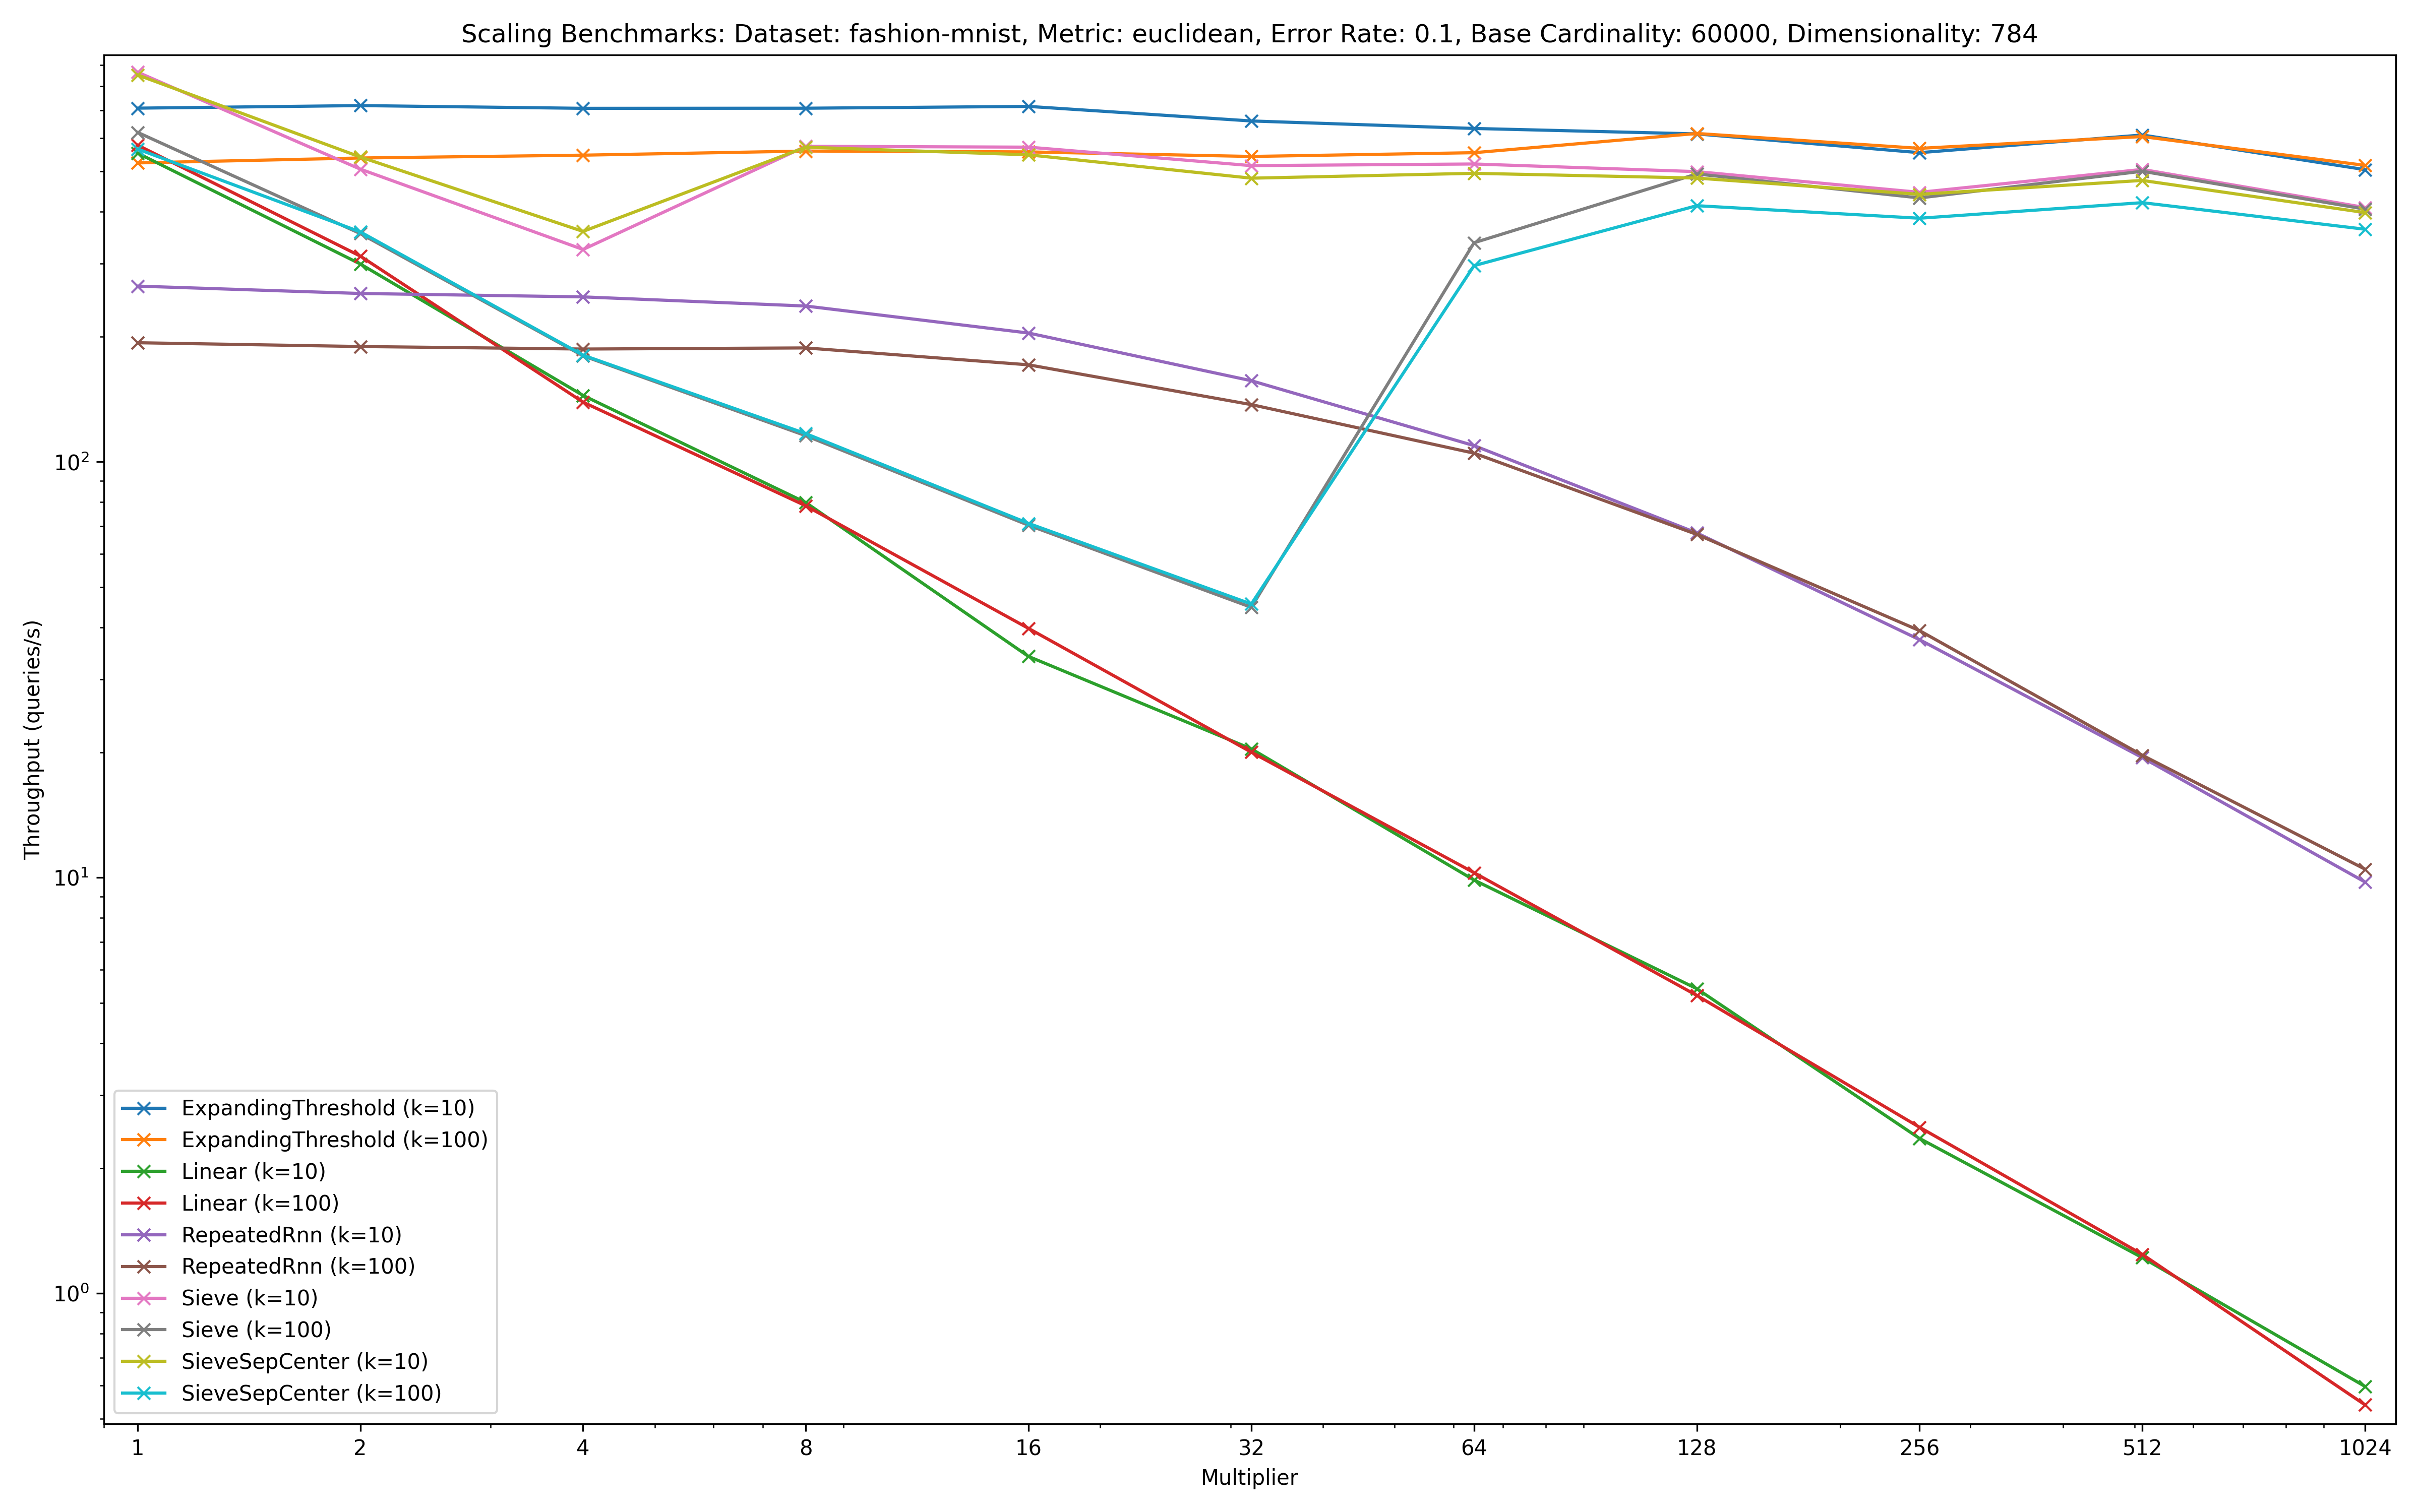
\includegraphics[width=3.4in]{images/result_plots/fashion-mnist_0.1_scaling.png}
    \caption{
        Fashion-mnist scaling
    }
    \label{fig:results:fashion-mnist-scaling}
\end{figure}

\begin{figure}[ht!]
    \centering
    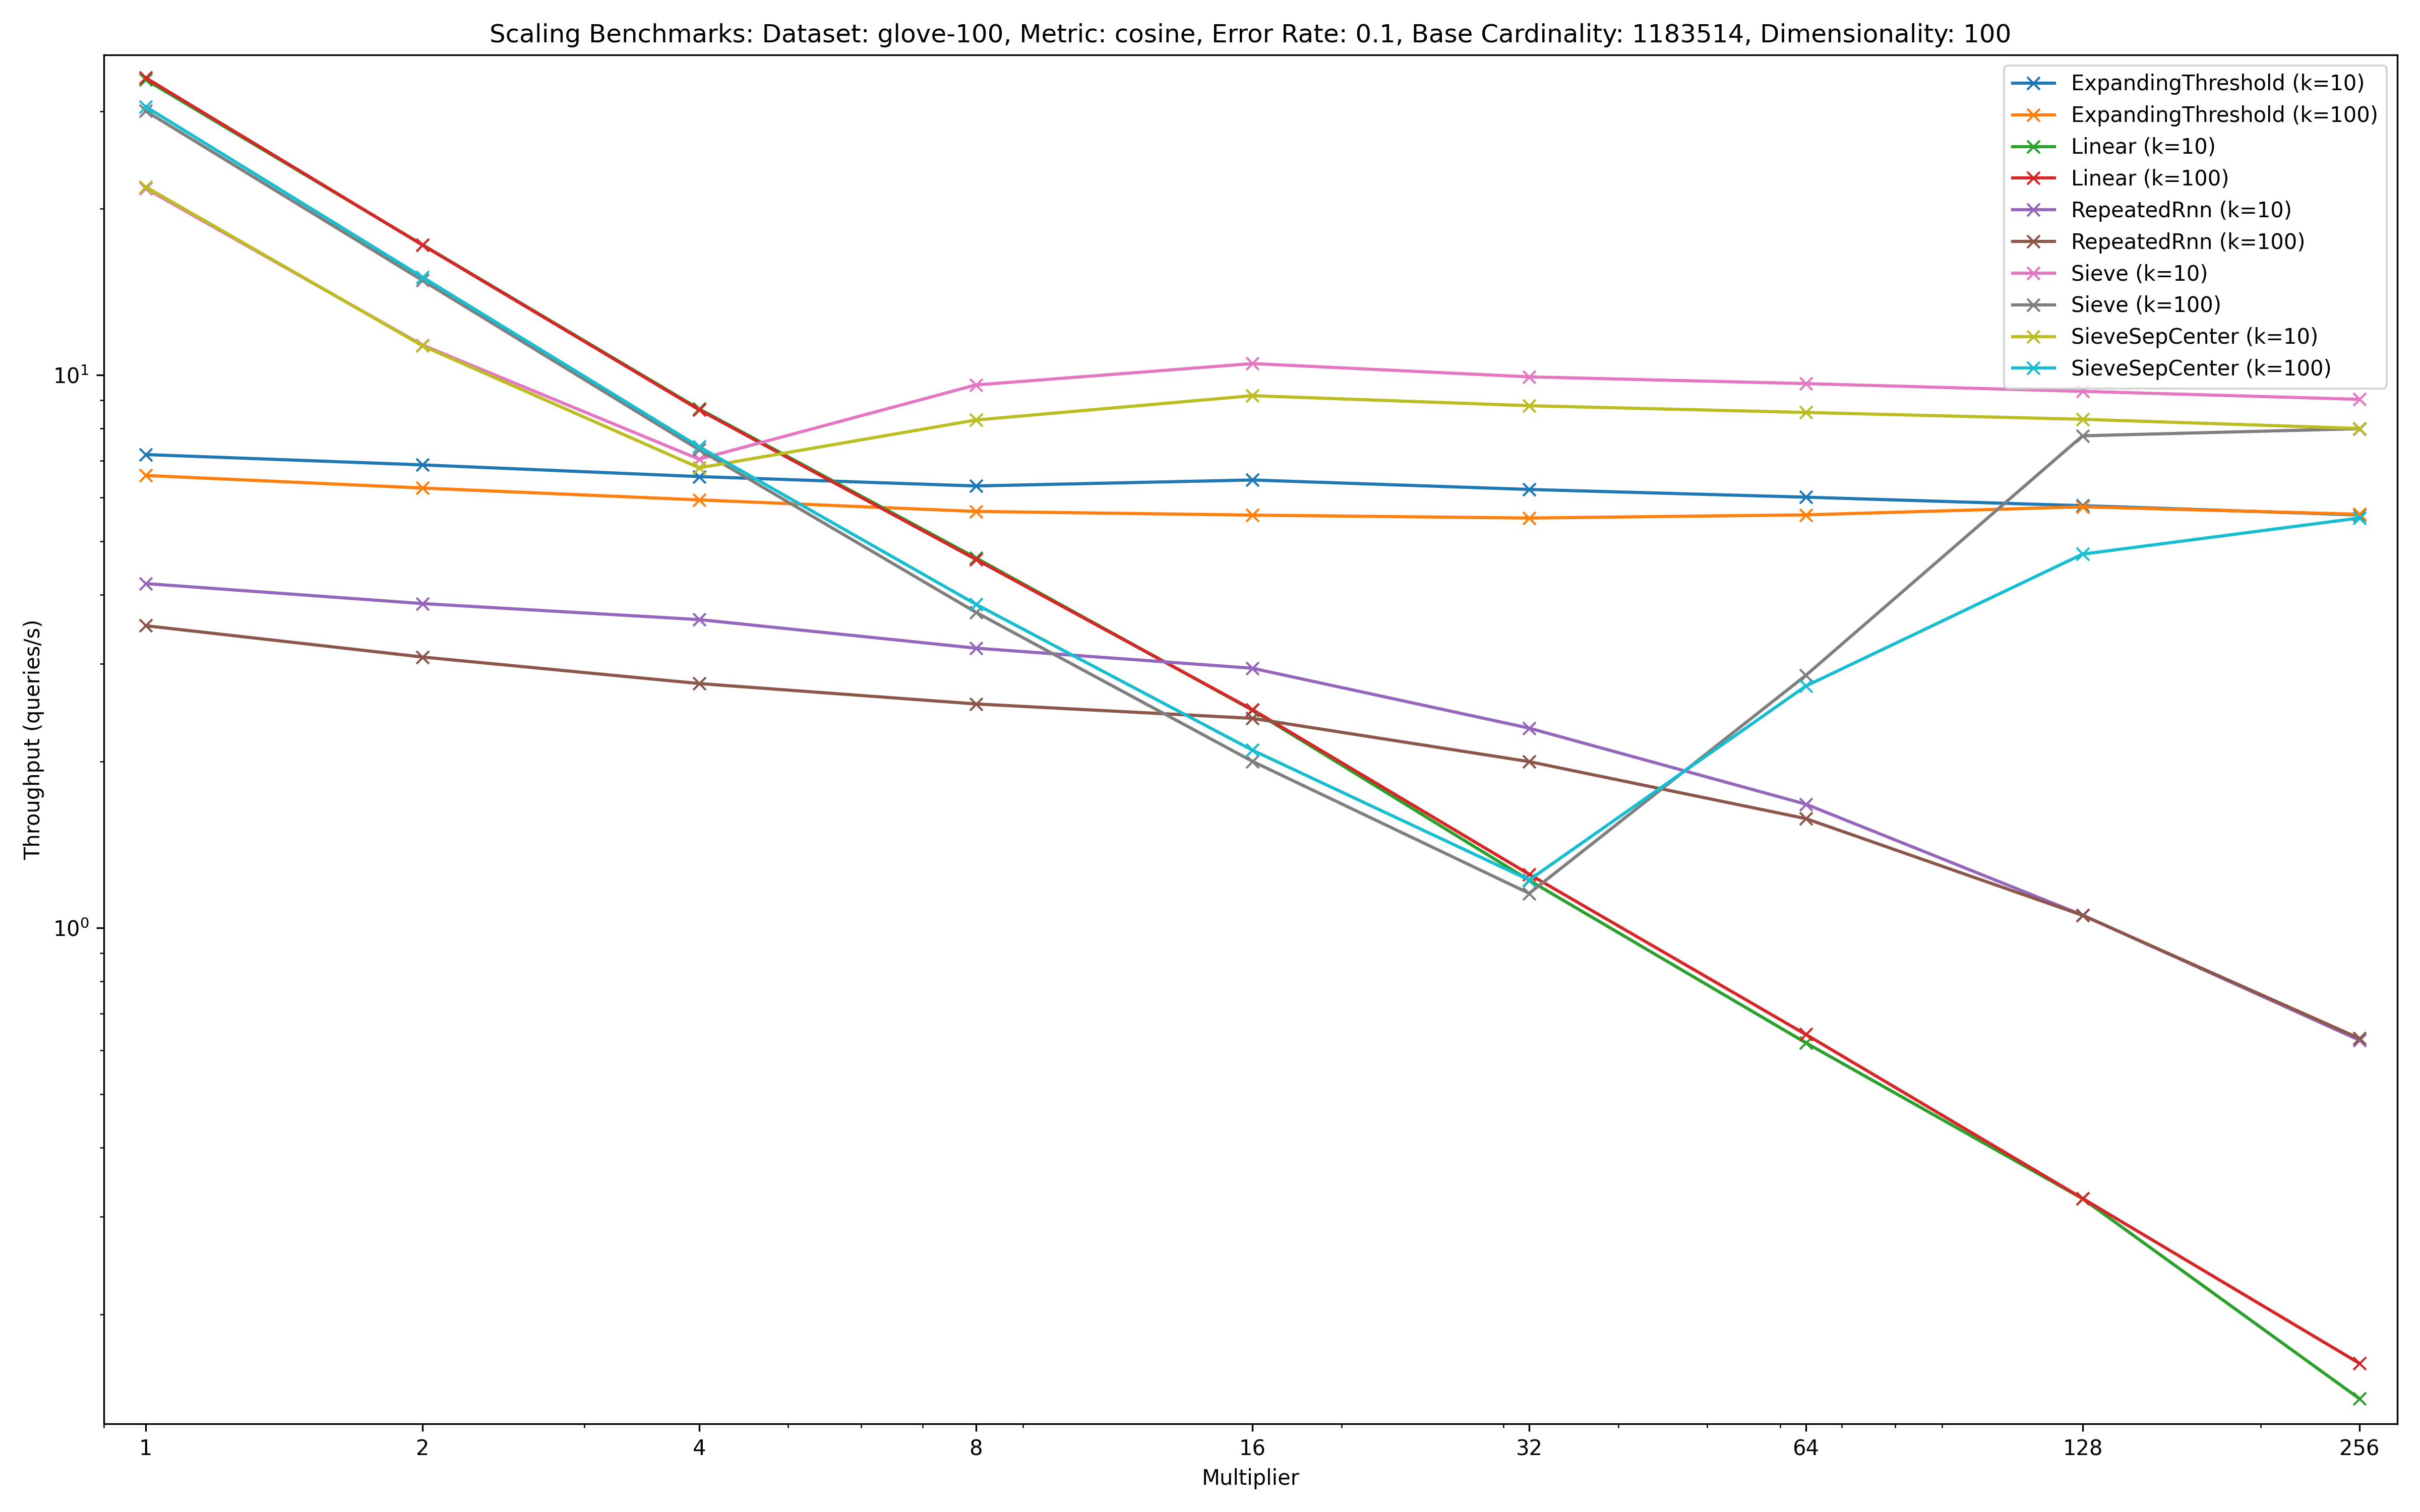
\includegraphics[width=3.4in]{images/result_plots/glove-100_0.1_scaling.png}
    \caption{
        Glove-100 scaling
    }
    \label{fig:results:glove-100-scaling}
\end{figure}


\begin{figure}[ht!]
    \centering
    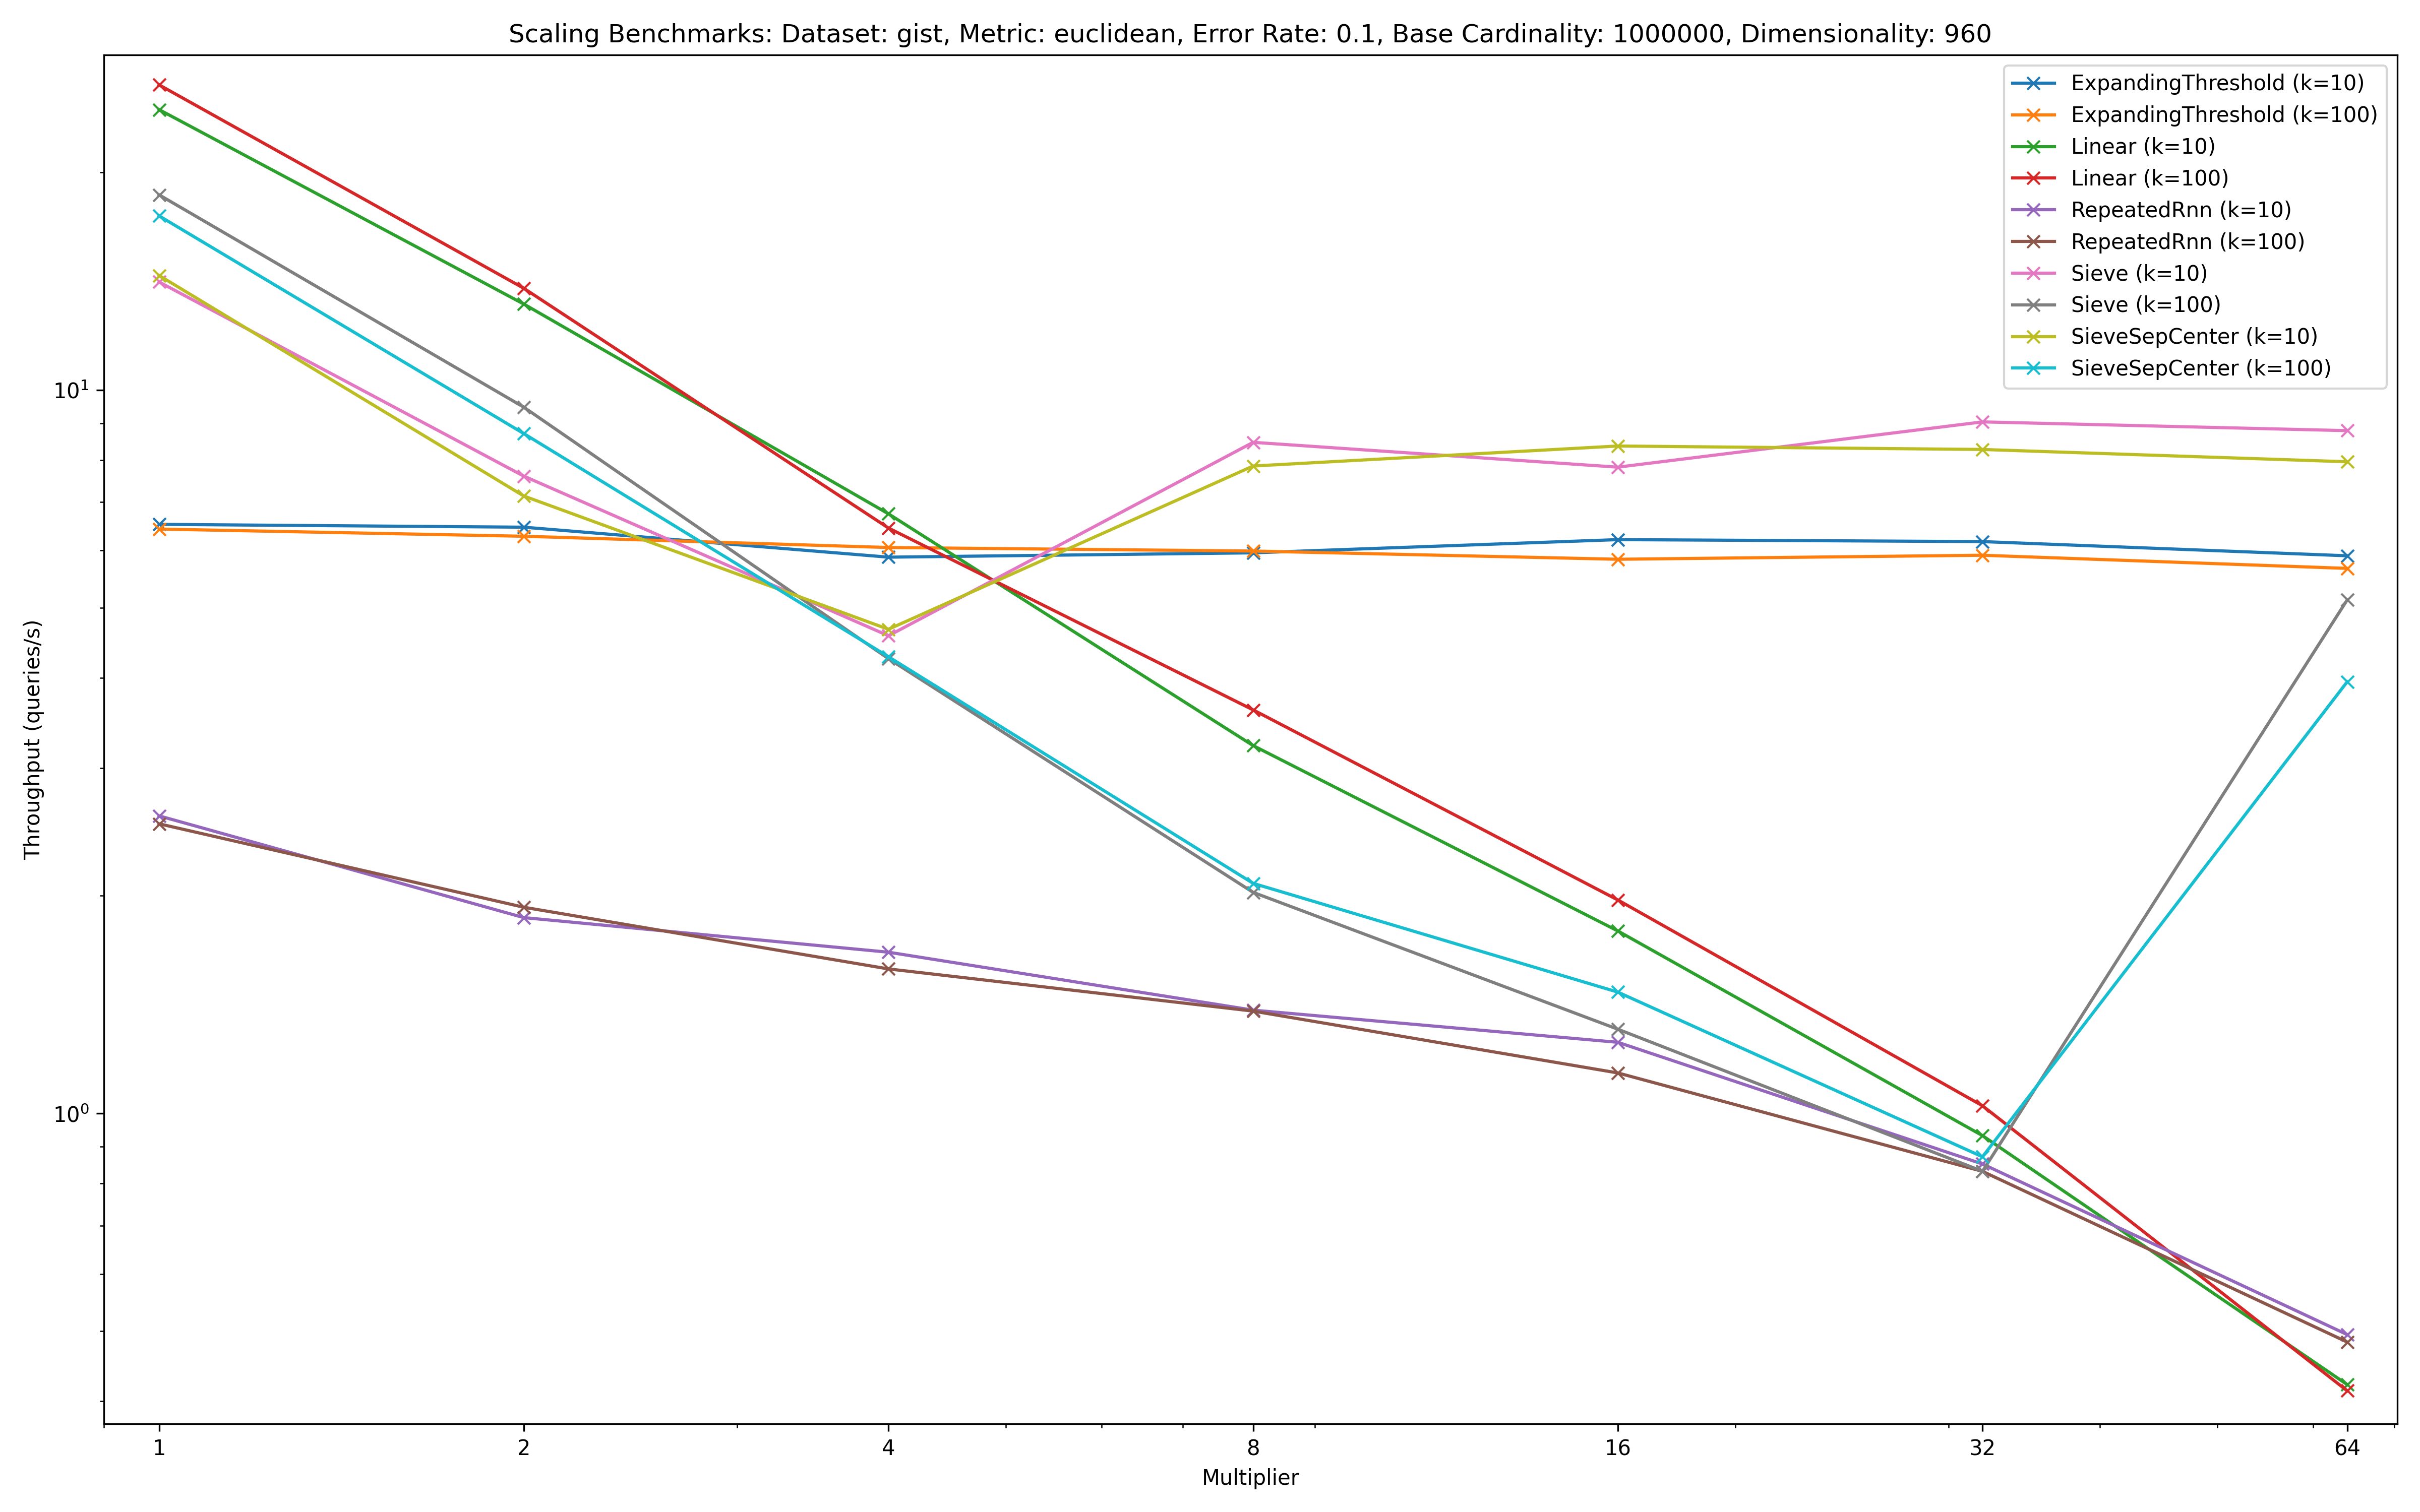
\includegraphics[width=3.4in]{images/result_plots/gist_0.1_scaling.png}
    \caption{
        Gist scaling
    }
    \label{fig:results:gist-scaling}
\end{figure}


\begin{figure}[ht!]
    \centering
    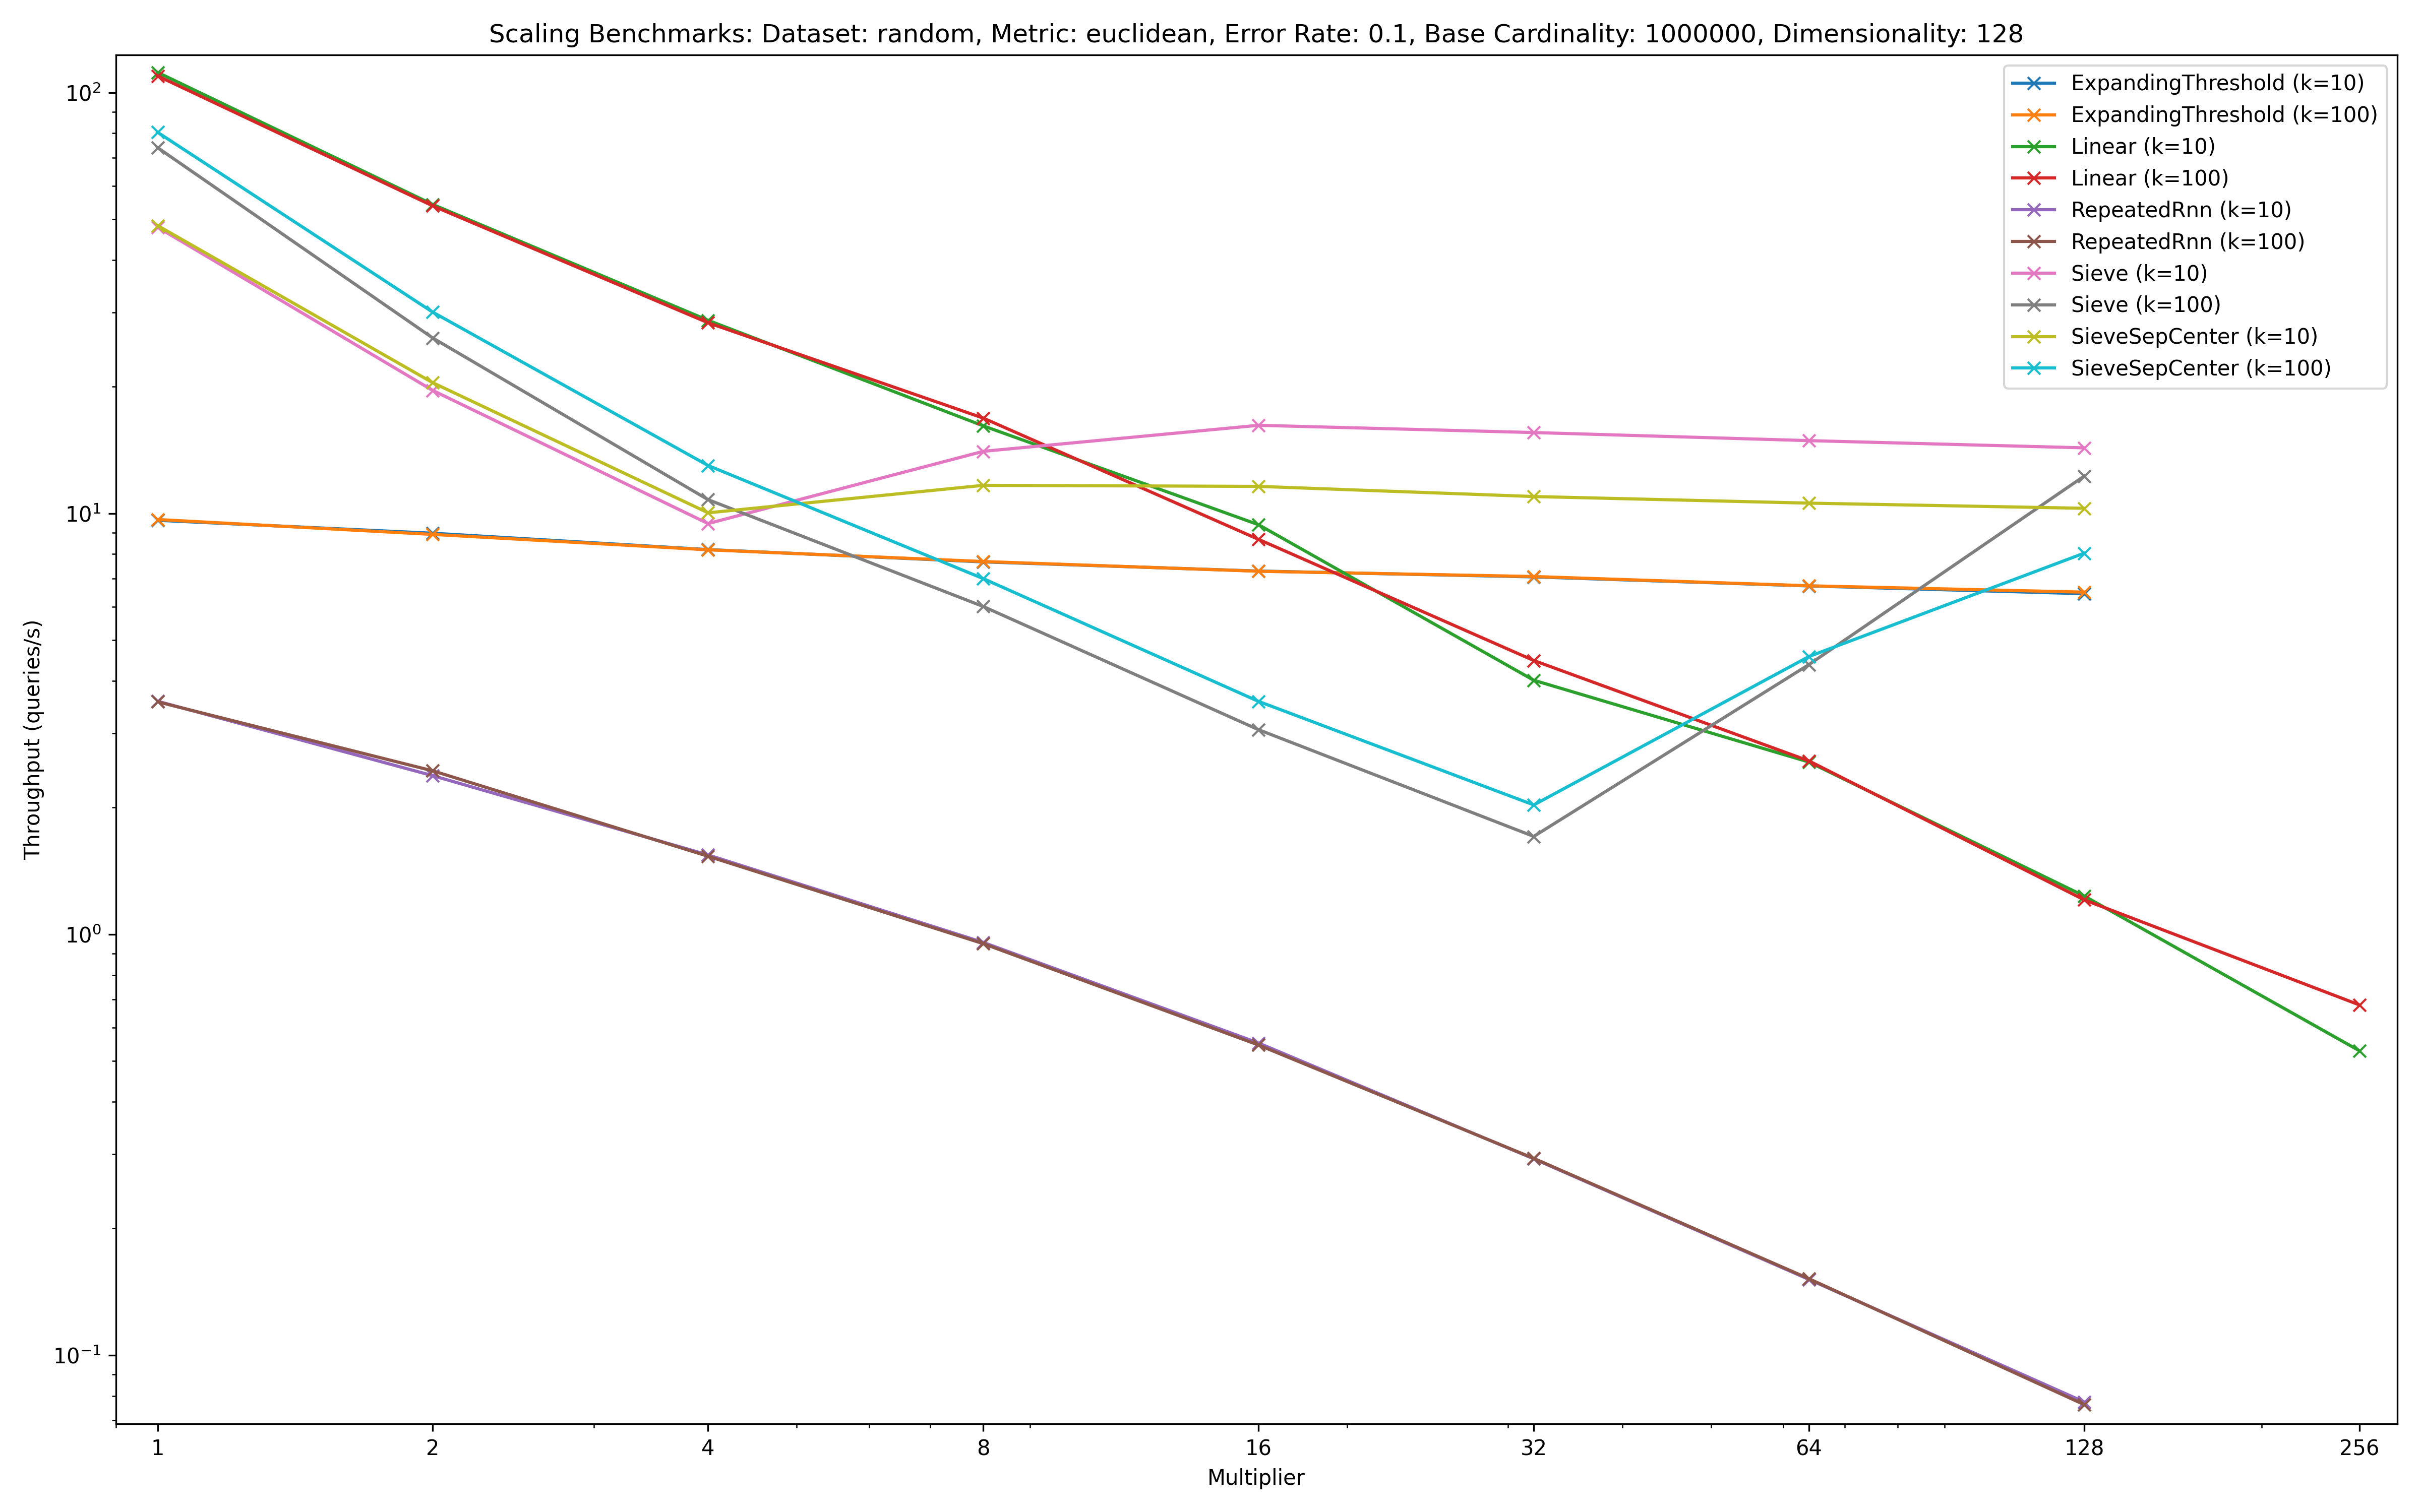
\includegraphics[width=3.4in]{images/result_plots/random_0.1_scaling.png}
    \caption{
        Random scaling
    }
    \label{fig:results:random-scaling}
\end{figure}

We stress that CAKES is intended for large datasets, and thus we do not expect to see sublinear performance on small datasets. 
To explore the scaling behavior of CAKES, we augmented datasets in the ANN-benchmarks suite by adding random points within a 
small error distance of existing points. This allowed us to isolate the effect of \emph{cardinality} on the performance of CAKES 
from that of other factors such as dimensionality, metric, or topological structure of the dataset. 


Figures \ref{fig:results:fashion-mnist-scaling}, \ref{fig:results:glove-100-scaling}, and \ref{fig:results:gist-scaling} show the scaling behavior of CAKES on augmented versions of the following ann-benchmark datasets: fashion-mnist under Euclidean distance, glove-100 under cosine distance, and gist under Euclidean distance. 
Figure \ref{fig:results:random-scaling} shows the scaling behavior of CAKES on a completely randomly generated dataset which does not obey any manifold structure. 
The the horizontal axes in each figure denote the multiplier by which the cardinality of the original dataset has been increased with synthetic points. The vertical axes denote throughput in queries per second, on a logarithmic scale. 


In Figure \ref{fig:results:fashion-mnist-scaling}, which shows results for fashion-mnist, we observe that as cardinality grows, all of our algorithms exhibit significantly better throughput than linear search. 
Of our algorithms, GreedySieve consistently performs best for both $k=10$ and $k=100$. For $k=10$, GreedySieve exhibits sublinear time performance for all cardinality multipliers, and for $k = 100$, GreedySieve begins to exhibit sublinear time performance at a relatively low multiplier (less than 1.5).  


For glove-100, as shown in Figure \ref{fig:results:glove-100-scaling}, we observe that all of our algorithms exhibit superior performance compared to linear search for large cardinalities. However, for $k=10$, linear search outperforms all of our algorithms until about a cardinality multiplier of 4, when Sieve and Sieve with Separate Centers begin to show superior performance. For $k=100$, this transition happens even later, at a mutliplier of about 6, when GreedySieve begins to have better throughput. 

With the notably adversial dataset gist, we observe that for $k=10$, three of our algorithms--GreedySieve, Sieve, and Sieve with Separate Centers--begin to outperform linear search at cardinality multipliers of aboyt 4, 6, and 6 respectively. 
For low values of $k$, Sieve and Sieve with Separate Centers appear to the be the best-performing algorithms. For $k=100$, we observe that GreedySieve significantly outperforms all other algorithms after a cardinality multiplier of 4. At multipliers lower than this threshold value, linear search exhibits the best throughput. With gist, unlike with the other datasets we benchmarked on, we see that RepeatedRnn (for both values of $k$), Sieve (for $k=100$), and Sieve with Separate Centers (for $k=100$) all show performance inferior to linear search even at high cardinalies. 

Figure \ref{fig:results:random-scaling} displays results for a random datset of base cardinality 1000000. 
These results illustrate the fact that absent a manifold structure in the dataset, it takes a much higher cardinality before CAKES begins to outperform linear search. 
In particular, for $k=10$, we see that Sieve is the best-performing method as cardinality grows, but that it only begins to outperform linear search after a multiplier of about 15. 
For $k=100$, we have that GreedySieve is the best-performing algorithm, but that it does not begin to have superior throughput until a multiplier of about 20. 
RepeatedRnn shows significantly worse performance on this dataset relative to both the other algorithms and to its own performance on real datasets. 
This is unsurprising, given that RepeatedRnn relies on a low local fractal dimension around the query in order to quickly zero in on the correct radius for $k$ hits. 
With a completely random dataset, which likely has much higher local fractal dimension, RepeatedRnn will meander for longer before finding this correct radius. 


Notably, we observe that on all datasets, GreedySieve's throughput stays nearly constant as cardinality increases. This observation warrants further investigation, but it is especially promising given that GreedySieve consistently outperforms linear search for high cardinalities and consistently outperforms our other algorithms for $k=100$. 
We also notice an interesting trend with Sieve and Sieve with Separate centers: for all datasets, at both values of $k$, both algorithms exhibit a sharp ``pivot point'' after which throughput starts to increase. 
While we observe that this pivot point seems to be proportional to the value of $k$, as it often occurs at about a multiplier of 4 when $k=10$ and a mulitplier of 32 when $k=100$, the reason for this behavior requires further investigation.  
Finally, we reiterate that the variation in performance across our algorithms based on dataset, value of $k$, and cardinality support our use of an autotuning function to select the best choice of algorithm. 
Currently, our autotuning function always uses $k=10$ for its determination, but our observation that the best algorithm differs significantly between small and large values of $k$ suggests that more sophisticated autotuning is necessary.


\subsection{Results against Competitors}

% We did not run any of the competitor's algorithms.
% We lifted the reported numbers from the ann-benchmarks site and their interactive plots.
% We made sure to use the same AWS instance as they did so it is a fair comparison.

% Tables \ref{table:results:ann-10} and \ref{table:results:ann-100} show the results of our benchmarks against FAISS, bruteforce-blas, and HNSW.
% The throughput values for these algorithms comes from the ANN benchmarks website's interactive plots, from which we can assess the throughput of each algorithm at a given recall value.

% We report the highest throughput value for each algorithm at a recall value of 1.0.
% We report the mean and median speedup factor of CAKES over each algorithm.
% For $k= 10$, we report a mean $7,654 \times$ (median $1,200 \times$) speedup over faiss-ivf, a mean $11,325 \times$ (median $2,821 \times$) speedup over bruteforce-blas, and a mean $485 \times$ (median $417 \times$) speedup over HNSW. 
% For $k=100$, we report a mean $4,479 \times$ (median $3,456 \times$) speedup over faiss-ivf, a mean $16,010 \times$ (median $13,548 \times$) speedup over bruteforce-blas, and a mean $403 \times$ (median $372 \times$) speedup over HNSW.

% For all datasets benchmarked in this manuscript, the auto-tuning method selected repeated $\rho$-nearest neighbor (Section~\ref{subsubsec:methods:knn-search:repeated-rnn}).

% We note that the mean and median speedup factors differ significantly for all methods, which suggests that the speedup factor is heavily dataset-dependent;
% in particular, across all algorithms, and both values of $k$, CAKES exhibits particularly high speedup factors with SIFT and GIST, under Euclidean distance.
% As GIST was designed to be a difficult dataset for classifiers~\cite{Lee2019PracticalLP}, CAKES's strong performance with this dataset is particularly encouraging.
% Further investigation of CAKES's performance on other challenging or adversarial datasets is warranted. 

% \begin{table*}[!t]
%     % \renewcommand{\arraystretch}{1.15}
%     \caption{Runtime performance (queries per second) of CAKES vs. other methods, $k=10$}
%     \label{table:results:ann-10}
%     \vskip 0.15in
%     \begin{center}
%         \begin{small}
%             \begin{sc}
%                 \begin{tabular}{|l|p{1cm}|p{1cm}|p{1cm}|p{1cm}|p{1cm}|p{1cm}|p{1cm}|p{1cm}|}
%                     \hline
%                     \textbf{Dataset}  & \multicolumn{2}{|c|}{\textbf{faiss-ivf}} & \multicolumn{2}{|c|}{\textbf{bruteforce-blas}} & \multicolumn{2}{|c|}{\textbf{hnsw(faiss)}} & \multicolumn{2}{|c|}{\textbf{CAKES}} \\
%                     \cline{2-9}
%                     &               Recall & QPS      & Recall & QPS    & Recall & QPS    & Recall & QPS \\
%                     \hline
%                     fashion-mnist & 1.000  & 188.03    & 1.000 & 52.91  & 1.000* & 339.74 & 1.000 & 141,800 \\
%                     \hline
%                     gist          & 1.000 & 3.55  & 1.000 & 2.63        & 0.953 & 149.58  & 1.000 & 76,420 \\
%                     \hline
%                     glove-25      & 1.000 & 78.78  & 1.000 & 33.52      & 1.000 & 552.67  & 0.798 & 94,580 \\
%                     \hline
%                     glove-100     & 1.000 & 21.16  & 1.000 & 16.52      & 0.998 & 155.90  & 0.904 & 4,566 \\
%                     \hline
%                     sift          & 1.000 &  24.52 & 1.000 & 16.40      & 1.000 & 275.07  & 1.000 & 357,400 \\
%                     \hline
%                 \end{tabular}
%             \end{sc}
%         \end{small}
%     \end{center}
%     \vskip -0.1in
% \end{table*}

% \begin{table*}[!t]
%     % \renewcommand{\arraystretch}{1.15}
%     \caption{Runtime performance (queries per second) of CAKES vs. other methods, $k=100$. Other methods did not report results for glove-25. Asterisk on recall value indicates that the algorithm had imperfect recall greater than or equal to 0.9995.}
%     \label{table:results:ann-100}
%     \vskip 0.15in
%     \begin{center}
%         \begin{small}
%             \begin{sc}
%                 \begin{tabular}{|l|p{1cm}|p{1cm}|p{1cm}|p{1cm}|p{1cm}|p{1cm}|p{1cm}|p{1cm}|}
%                     \hline
%                     \textbf{Dataset}  & \multicolumn{2}{|c|}{\textbf{faiss-ivf}} & \multicolumn{2}{|c|}{\textbf{bruteforce-blas}} & \multicolumn{2}{|c|}{\textbf{hnsw(faiss)}} & \multicolumn{2}{|c|}{\textbf{CAKES}} \\
%                     &                    Recall & QPS  & Recall & QPS     & Recall & QPS      & Recall & QPS \\
%                     \hline
%                     fashion-mnist  & 1.000 & 111.47    & 1.000* & 16.02   & 1.000* & 277.80   & 1.000 & 71,370 \\ 
%                     \hline
%                     gist           & 1.000 & 2.70      & 1.000* & 0.80    & 0.995 & 59.71     & 1.000 & 29,090 \\
%                     \hline
%                     glove-25       & -- & --           & --     & --      & -- & --           & 0.851 & 49,350 \\
%                     \hline
%                     glove-100      & 1.000* &  19.04   & 1.000* & 7.52    & 0.987 & 92.58     & 0.905 & 4,384 \\
%                     \hline
%                     sift           & 1.000 &  23.50    & 1.000  & 6.51    & 1.000* & 179.14   & 1.000 & 147,400 \\                                                 
%                     \hline
%                 \end{tabular}
%             \end{sc}
%         \end{small}
%     \end{center}
%     \vskip -0.1in
% \end{table*}


% \begin{table*}[!t]
%     % \renewcommand{\arraystretch}{1.15}
%     \caption{Runtime performance (queries per second) of CAKES and Speedup Factor over Naive Linear Search, $k=10$}
%     \label{table:results:ann-alt-10}
%     \vskip 0.15in
%     \begin{center}
%         \begin{small}
%             \begin{sc}
%                 \begin{tabular}{|l|l|l|l|l|}
%                     \hline
%                     \textbf{Dataset} & \textbf{CAKES Throughput} & \textbf{Speedup Factor over Linear} \\
%                     \hline
%                     deep-image       & 232.1                     & 37.2      \\
%                     \hline
%                     mnist            & 129,300                   & 101.9      \\
%                     \hline
%                     glove-50         & 10,950                    & 12.28      \\
%                     \hline 
%                     glove-200        & 2,290                     & 8.55     \\
%                     \hline
%                     lastfm           & 13,950                    & 4.55           \\
%                     \hline
%                 \end{tabular}
%             \end{sc}
%         \end{small}
%     \end{center}
%     \vskip -0.1in
% \end{table*}


% \begin{table*}[!t]
%     % \renewcommand{\arraystretch}{1.15}
%     \caption{Runtime performance (queries per second) of CAKES and Speedup Factor over Naive Linear Search, $k=100$}
%     \label{table:results:ann-alt-100}
%     \vskip 0.15in
%     \begin{center}
%         \begin{small}
%             \begin{sc}
%                 \begin{tabular}{|l|l|l|l|l|l|}
%                     \hline
%                     \textbf{Dataset} & \textbf{CAKES Throughput} & \textbf{Speedup Factor over Linear} \\
%                     \hline
%                     deep-image        & 157.3                    & 25.74                               \\                            
%                     \hline
%                     mnist             & 71,090                   & 56.63                               \\
%                     \hline
%                     glove-50          & 8,867                    & 9.84                                \\
%                     \hline 
%                     glove-200         & 2,264                    & 8.49                                \\
%                     \hline
%                     lastfm            & 13,950                   & 4.55                                \\
%                     \hline
%                 \end{tabular}
%             \end{sc}
%         \end{small}
%     \end{center}
%     \vskip -0.1in
% \end{table*}
